%Créé par Claudine Allen en collaboration avec Jean-Raphaël Carrier
%Dernière modification JRC: 13 janvier 2014
%Élimination du labo de résistivité des matériaux (IV) à la fin de l'ère JRC + regroupement des labos VI & VII en début de pandémie COVID-19 => renumérotation IX -> VII maintenant
%Dernière modification CA: 14 novembre 2023
%Dernière modification JG:
%***ToDo***
% - préparer un signal de bruit pour montrer comment on se rapproche de sinus/cosinus avec Q qui augmente dans un filtre passe-bande,... voir version JG.
% -  recopier préparation & déroulement de l'atelier en ordre inverse en ligne dans le cours 6.

\RequirePackage[l2tabu, orthodox]{nag} %Check for obsolete commands
\documentclass[canadien,12pt,oneside,letterpaper]{article}
%
%-----------------------------------------------------
%Loading packages
%
\usepackage[utf8]{inputenc}
\usepackage[T1]{fontenc}
\usepackage[canadien]{babel}
\usepackage{lmodern}
\usepackage{textcomp}
\usepackage{amsmath,amssymb}
\usepackage{siunitx}
\usepackage{xcolor}
\usepackage[colorlinks=true,allcolors=blue]{hyperref}
\usepackage[all]{hypcap}
\usepackage{graphicx}
\usepackage[americanvoltages,americancurrents,siunitx]{circuitikz}
\usetikzlibrary{babel}
\usepackage{caption}
\usepackage{subcaption}
%\usepackage{subfig}
\usepackage[letterpaper,headheight=15pt]{geometry}
\usepackage{fancyhdr}
\usepackage{setspace}
%
%----------------------------------------------------
%Other configurations and layout
%
\sisetup{separate-uncertainty}
\captionsetup{font=small,labelfont=bf,margin=0.1\textwidth}
\pagestyle{fancy}
\fancyhf{}
\lhead{\textsl{GPH-2006/PHY-2002~---~Laboratoire~VII}}
\rhead{\textsl{Page \thepage}}
\setcounter{secnumdepth}{0}
\setlength{\parskip}{1.5ex plus0.5ex minus0.2ex}
%\onehalfspacing
\interfootnotelinepenalty=10000 %To avoid footnotes spreading on several pages.
%
%---------------------------------------------------
%
\title{\textbf{Atelier VII}\\Filtres passifs \& actifs\thanks{Auteurs: Claudine Allen, Samuel Nadeau \& Jean-Raphaël Carrier \& Jérémie Guilbert}}
\renewcommand\footnotemark{}
\date{}


\begin{document}

\maketitle \vspace{-2cm}

\noindent\textit{\textbf{Prélude de contexte et déroulement des ateliers}}

\textit{Les ateliers se rapprochent d'un mode de travail expérimental plus autonome, s'éloignant du contexte pédagogique pour se rapprocher du milieu professionnel. En effet, après avoir étudié tous les éléments de la section \nameref{sec:lectures}, vous devez concevoir votre propre protocole dans votre cahier de recherche afin d'atteindre les objectifs de chaque partie. Les questions à explorer et la section \nameref{sec:prep} vous guideront dans votre rédaction du protocole, puis l'équipe d'enseignement vous assistera au laboratoire avec toute explication souhaitée et des suggestions pour bonifier vos manipulations. S'il reste du temps à la fin de chaque atelier, profitez-en pour avancer votre projet de conception final afin de mieux respirer en fin de session et de bénéficier directement de support de l'équipe.}

\textit{Les équipes pour ces ateliers et le projet de conception passent de 2 à 4 personnes pour partager les tâches de modélisation, conception et simulation en plus des manipulations expérimentales, des mesures à prendre et de leur analyse. Vous pouvez même utilisez des postes et plaquettes de montage en parallèle afin que personne ne se tourne les pouces! Consignez soigneusement tout votre travail dans votre cahier de recherche et assurez-vous que le superviseur de l'équipe d'enseignement qui vous encadre évalue si vous avez atteint les objectifs avant de démonter vos circuits. Il n'y a aucune autre remise à faire pour les ateliers afin de vous donner le temps de travailler sur votre projet final.}


\vspace{-2.5ex}
\section{Thématique}\label{sec:theme}
\vspace{-1.5ex}
Une fonction essentielle accomplie par des circuits électriques dans le travail expérimental est celle de filtrer un signal. En télécommunications par exemple, le concept de filtrage est à la base de la décryption des signaux. Plus généralement, il est également possible d'utiliser les filtres pour retirer des fréquences indésirables et généralement obtenir des mesures plus fidèles avec un meilleur rapport signal sur bruit. L’effet de filtres sur le gain et la phase de signaux en tension sera donc étudié dans ce laboratoire à l’aide du diagramme de Bode. En particulier, les performances de différents design de filtres avec des composants uniquement passifs seront comparées à un design intégrant un amplificateur opérationnel actif. Ce laboratoire, en association avec le deuxième devoir, a aussi pour objectif d’approfondir la compréhension de l’étudiant.e des domaines temporel et fréquentiel dans le cadre des transformations de Laplace et Fourier. La relation entre délai temporel et déphasage sera donc aussi examinée pour le filtre RC.\\

%Les travaux effectués aborderont les objectifs d’ensemble 1, 2, 4, 5, 7, 9, 10, 11 et 12 du plan de cours + BAIC?
\vspace{-2ex}
\section{Lectures préparatoires}\label{sec:lectures}

\begin{itemize}
\item cours \textit{Analyse de circuits résistifs et réactifs}, votre compréhension des expériences sera largement supérieure en ayant étudié ce cours avant le laboratoire!
\item complément \textit{Analyse temporelle}
\item complément \textit{Analyse fréquentielle}
\end{itemize}


\vspace{-2ex}
\section{Préparation}\label{sec:prep}
%Est-ce qu'on donne du pointage de préparation, surtout ici qu'on devrait vérifier qu'il ont écouté le cours en ligne...
\vspace{-3ex}
AVANT la séance d'atelier, écrivez sommairement dans votre cahier de recherche tout ce que vous prévoyez faire au laboratoire pour atteindre les objectifs. N'oubliez pas de calculer toute valeur ou modèle de référence donné en complément aux fins de comparaison à l'expérience. En plus des manipulations expérimentales, des mesures à prendre et de leur analyse, notez aussi les étapes de modélisation, conception et simulation nécessaires. Plusieurs logiciels spécialisés pour l'électronique listés sur le site de cours, dans la section \texttt{Logiciels} de l'onglet \texttt{Matériel didactique}, vous aideront dans cette préparation. En particulier, l'onglet \texttt{Circuits} de \href{https://www.falstad.com/circuit/}{l'application Web de Paul Falstad} contient pratiquement tous les circuits en atelier, montrant directement les comportements idéaux attendus\footnote{Une liste des circuits se trouve \href{https://www.falstad.com/circuit/directions.html}{ici} et des réponses en fréquence (diagrammes de Bode du gain) de différents filtres selon le menu \texttt{Circuits} sont même disponibles \href{https://www.falstad.com/afilter/}{ici}. N'hésitez pas à explorer les possibilités du menu \texttt{Dessiner~>~Sorties et étiquettes} de l'app, entre autres pour exporter des données de simulation.}. Comme la programmation LabVIEW s'avère souvent chronophage, vous pouvez être soulagés qu'aucun VI n'est demandé pour les ateliers. Toutefois pour mieux caractériser les filtres avec des diagrammes de Bode, utilisez le VI LabVIEW déjà prêt dans le module de cet atelier.

\section{Partie 1}\label{sec:analyseRC}
Les objectifs à atteindre avec le filtre RC de la figure~\ref{fig:passe-bas-RC} sont :

\begin{itemize}
    \item associer les domaines temporel et fréquentiel en faisant théoriquement et expérimentalement son analyse par transformée de Laplace et Fourier,
    \item améliorer son fonctionnement pour le rapprocher d'un filtre idéal indépendant de la charge placée à sa sortie.
\end{itemize}

\begin{figure}[h]
\centering
\begin{circuitikz} \draw
(0,2) node[left]{$v_{\mathrm{in}}$} to[R=1~k$\Omega$,o-] (3,2) to[short,-o] (4,2) node[right]{$v_{\mathrm{out}}$}
(3,2) to[C=1~$\mu$F] (3,0) node[ground]{}
;\end{circuitikz}
\caption{\label{fig:passe-bas-RC}Circuit RC série.}
\end{figure}

\subsection{Questions à explorer avec ce circuit}
\begin{itemize}
    \item Comment se comparent quantitativement les diagrammes de Bode obtenus théoriquement à ceux mesurés expérimentalement à l'aide du VI sur le site de cours (voir les instructions ci-dessous)? %viser comparaison quantitative avec soustraction et genre somme des résidus carrés pour comparaison
    %\item Par rapport à la fréquence de coupure, sur quelle plage fréquentielle la phase du signal en sortie $v_{\mathrm{out}}$ est en avance sur celui en entrée $v_{\mathrm{out}}$? Et puis sur quelle plage est-il en retard? %peufiner pour mettre en relief le passage du délai à déphasage
    \item Quel(s) signal(aux) du générateur de fonctions vous permettrait(ent) de quantifier directement à l'oscilloscope le délai causé par le filtre? Quels sont des paramètres que vous pouvez mesurer pour ce faire?
    \item Est-ce que le produit $RC$ pour ce filtre correspond à la constante de temps mesurée avec le signal choisi? Évaluez l'inverse de cette constante et retrouvez la valeur de gain correspondante sur votre diagramme de réponse en fréquence, quel est son écart par rapport à la valeur idéale de 0.5 ? %vériiier que c'est -6dB et ajouter entre parenthèses
    \item Que se passe-t-il si vous inversez le condensateur et la résistance? Expliquez d'où vient ce changement de comportement.
    %\item question de vérification de disparition de la réponse transitoire à une impulsion -> réponse impulsionnelle après une temps > à un certain nombre de constantes RC
    \item Calculez et/ou examinez directement à l'oscilloscope la transformée de Fourier d'un signal carré. Quelle est une fréquence de ce signal qui permet d'éliminer plusieurs harmoniques tout en préservant la fondamentale avec le filtre? Vérifiez-le expérimentalement et observez aussi le signal filtré qui en résulte dans le domaine temporel. %P-e jouer aussi avec l'applet Falstad qui "compose" des signaux.. & Voir si on ne peut pas faire PWM avec différents duty cycles (en le définissant) au générateur, ça aiderait pour l'utilisation de l'arduino et pourrait segway à l'oscillateur à relaxation qui fait du siswitching comme ça non? Changer le duty cycle avec un potentiomètre possible?
    \item Placez une charge de 1~k$\Omega$ à la sortie du filtre pour représenter l'application utilisant le signal, comment ce dernier est-il affecté? Est-ce que l'ajout d'un composant étudié au dernier laboratoire pourrait régler ce problème? Faites le test de votre hypothèse. 
    \item Branchez une réplique du filtre original à la sortie au lieu de la résistance, de quelle manière ce filtre est alors amélioré? Décrivez ce qui se produit si vous enlevez le composant actif. Notez que vous pouvez continuer de cascader des filtres ainsi pour optimiser le filtrage et le nombre de cascades est alors défini comme l'ordre du filtre complet.  %Pente de "roll-off" de 20n dB/decade \approx 6n dB/octave, où n est l'ordre du filtre, "cutoff" reste à un gain de 0.5
    \item Pensez-vous que remplacer le condensateur par une bobine d'inductance améliorerait les performances de filtrage? %sonne un peu familier? utiliser le mot hypothèse? Éléments de réponse : Théoriquement ce serait le même comportement idéal, mais L'inductance fait des courts-circuits à basse fréquence, donc marche bien juste pour haute fréquence -> doit fitter avec coupure (mais induit alors de forts champs magnétiques->bruit d'ondes EM) et doit protéger le circuit pour les basses fréquences. Condensateur est ouvert aux basses férquences et c'est rare qu'on va à d'assez hautes fréquences pour le court-circuiter! Aussi de Wiki: "A first-order RL circuit is one of the simplest analogue infinite impulse response electronic filters. It consists of a resistor and an inductor, either in series driven by a voltage source or in parallel driven by a current source."
    %\item calcul d'impédance d'entrée et de sortie de filtre, à mieux définir par rapport à ce qui constitue entrée et sortie en complément (même faire pour amplification au lab VI et répéter ici)
\end{itemize}

\subsubsection{Instructions pour le VI d'acquisition des diagrammes de Bode}
Les diagrammes de Bode nécessitent une fréquence idéalement unique en abscisse, ce qui est obtenu expérimentalement avec un signal sinusoïdal envoyé par le générateur de fonctions. Branchez ce signal de tension sur le canal~1 de l'oscilloscope et à l'entrée du filtre alors que celui à sa sortie sera lu en l'envoyant au canal~2. Sur la face-avant du VI, faites en sorte que les types des mesures 1, 2 et 3 soient respectivement \texttt{Amplitude}, \texttt{Amplitude} et \texttt{Phase}. La fréquence initiale $f_{\mathrm{ini}}$ doit être 1~Hz. Fixez le nombre d'itérations à 25. Les mesures seront prises une fois par octave, \textit{i.e.} aux fréquences définies par $f_{i}=2^i\,f_{\mathrm{ini}}$, donc de 1~Hz à 16,777~MHz (soit presque la totalité de la plage de l'oscilloscope). Lorsque vous tracerez les diagrammes de Bode, ne prenez pas en compte les points où la valeur est de 9,90E+37 ; ces mesures sont erronées et sont dues au fait que le signal à cette fréquence était trop faible pour une mesure adéquate avec l'oscilloscope. %Mettez $V_{\mathrm{min}}$ à $-2$~V et $V_{\mathrm{max}}$ à 2~V, mais il fallait changer pour certains filtres dans la version "laboratoire" anyway.

\section{Partie 2}\label{sec:conceptionRLC}
L'objectif de cette partie est de concevoir et analyser un filtre passe-bande selon la configuration de la figure~\ref{fig:passe-bande-RLC} qui doit répondre aux spécifications demandées.
%Calculateur http://sim.okawa-denshi.jp/en/RLCtool.php and find back the French one
\begin{figure}[h!]
\centering
\begin{circuitikz} \draw
(0,2) node[left]{$v_{\mathrm{in}}$} to[L,l=$L$,o-] (2.5,2) to[C,l=$C$] (5,2) to[short,-o] (6.5,2) node[right]{$v_{\mathrm{out}}$}
(5.5,2) to[R,l_=$R$] (5.5,0) node[ground]{}
;\end{circuitikz}
\caption{Filtre RLC série.}
\label{fig:passe-bande-RLC}
\end{figure}

\subsection{Questions à explorer avec ce circuit}
\begin{itemize}
    \item Quels composants dans votre coffre permettent d'obtenir une fréquence naturelle de résonance $f_0$ d'environ 5033 Hz? %Réponse possible : L= 1 mH (10e-3), C= 1 microfarad (10e-6)
    \item Quelle valeur de résistance dissipative peut alors élargir la bande passante $B$ à 42972 Hz? %Réponse possible : R= 270 ohms
    \item Est-ce que le circuit réalisé avec ces composants montre bien la réponse en fréquence prévue? %Pour le déphasage, je pourrais amener mon idée de comparer à un système masse-ressort en jeu de raquette-balle qu'on voit clairement en phase à basses fréquence et déphasé de pi (ou pi/2) en résonance et perd tout après!!! OU garder pour les oscillateurs???
    \item Quel est le facteur de qualité $Q=f_o/B$ de ce résonateur? %Réponse correspondante : Q=0.117
\end{itemize}
%Réponse possible : L= 1 mH (10e-3), C= 1 microfarad (10e-6), R= 270 ohms
%RLC générique, setter RLC
% De la mesure de SNR pourrait être ramenée à qqpart dans le coin avec carré des résidus par rapport à une référence qui devient le bruit.

\section{Partie 3}\label{sec:filtrage-source}
 L'objectif final de cet l'atelier est d'adapter un filtre des parties précédentes pour décrypter le signal qui vous est fourni via un module Moku: Go selon les instructions à la fin de cette partie.

\subsection{Questions à explorer avec votre circuit}
\begin{itemize}
    \item Pouvez-vous vérifier que les fréquences dominantes dans le signal crypté correspondent bel et bien à celles présentes dans le code Python; soit 50 Hz et 1000 Hz?
    \item Quel type de circuit avez-vous besoin de créer pour décoder le signal de sorte qu'on isole la partie qui possède une fréquence basse? Quel sera la valeur nominale initialement choisie pour chaque composant de votre filtre? 
    \item En testant quelques autres valeurs pour les composants de votre circuit, vérifiez si le décryptage du signal est bel et bien optimal avec les valeurs initiales calculées. Si ce n'est pas le cas, quels facteurs peuvent avoir causé cette différence?
    \item À quel point votre circuit est-il efficace pour décoder le signal? Décrivez qualitativement. 
    %\item En utilisant le code LabView pour faire un diagramme de Bode, pouvez-vous déterminer la réponse en fréquence de votre circuit? Caractérisez celle-ci.
    \item Quels améliorations ou changements peuvent être faits au circuit pour mieux décrypter le signal?
\end{itemize}

\subsubsection{Instructions pour la génération de signal avec le Moku: Go}
Commencez par alimenter le Moku: Go et branchez-le dans votre ordinateur avec le cable USB-C. Ensuite, ouvrez l'application \texttt{Moku} et attendez que celle-ci détecte l'instrument. Le processus peut prendre jusqu'à environ deux minutes donc soyez patient. Lorsque vous voyez apparaître l'icône du Moku: Go, faites un clic droit sur celle-ci pour obtenir une copie de son adresse réseau IP en sélectionnant \texttt{device info $\rightarrow$ Copy IP address} tel qu'illustré à la figure~\ref{fig:MokuIP}.

\begin{figure}[h]
\centering
    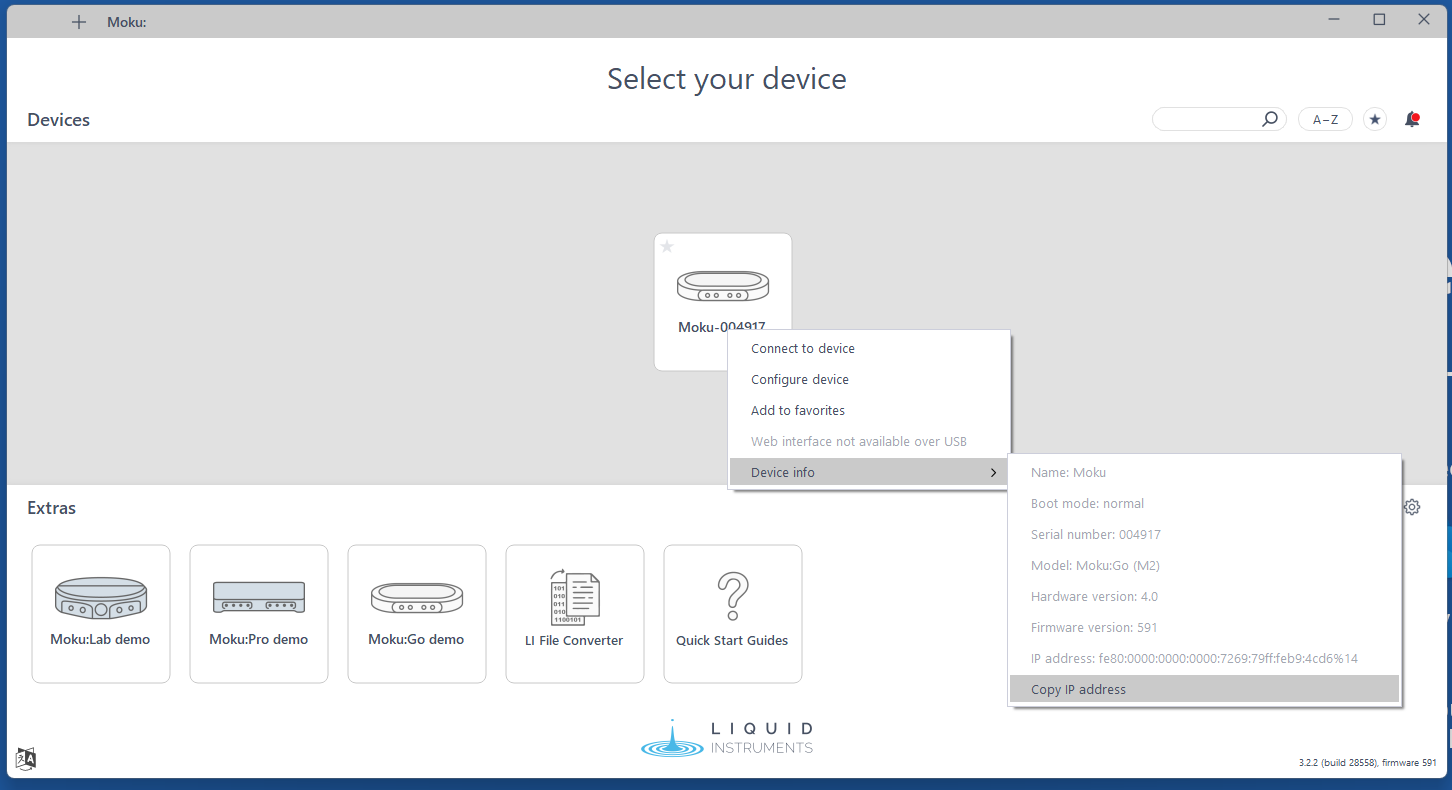
\includegraphics[scale=0.35]{MokuTuto3.png}
    \caption{Menu pour obtenir l'adresse IP identifiant votre Moku : Go.}
    \label{fig:MokuIP}
\end{figure}

Maintenant, il ne reste qu'à coller l'adresse IP dans le script Python à télécharger du site de cours. Remplacez l'adresse qui est déjà présente dans le code, en vous assurant de la mettre à l'intérieur des crochets comme surligné dans la figure~\ref{fig:MokuScript}.

\begin{figure}[h]
\centering
    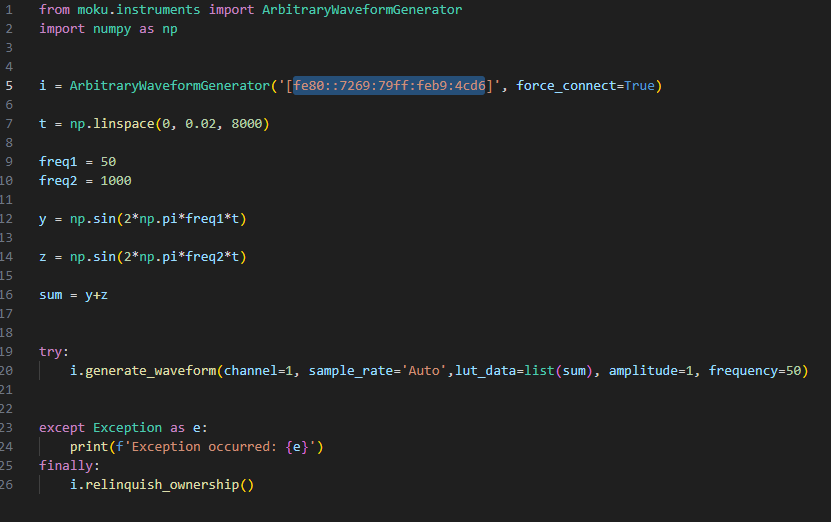
\includegraphics[scale=0.6]{MokuTuto4.png}
    \caption{Script Python faisant appel au module API Moku afin de générer un signal.}
    \label{fig:MokuScript}
\end{figure}

Vous pouvez maintenant exécuter le code pour générer le signal à la sortie~1 du Moku : Go.

\end{document}

% Les sources à filtrer construites par Daniel :)
% \begin{enumerate}
% \item Une source "constante", qui varie lentement. Vous devez concevoir un filtre pour la stabiliser tout en gardant la tension lorsqu'une charge de 1 kOhms  est connectée.
% \item Une source sinusoidale bruyante. Vous devez concevoir un filtre pour enlever le bruit hautes fréquences tout en gardant la tension lorsqu'une charge de 1 kOhms est connectée.
% \item Une source analogique "constante" comme on trouve sur les Arduinos, de type Pulse Width Modulation. Vous devrez faire un filtre passe-bas qui fonctionnera, quelle que soit la résistance de charge utilisée, pour obtenir une tension proportionnelle constante.
% \end{enumerate}

%Le filtrage proposé par Jérémie :
\section{Filtrage d'une source}
% Maintenant que vous avez déterminé les spectres du gain des filtres de la figure \ref{sch-RC-ordre3}, mettez-les à l'épreuve en les utilisant pour retirer les hautes fréquences d'un signal bruité. Pour ce, utilisez le générateur de fonctions d'un oscilloscope afin d'envoyer un signal de type \textit{bruit} dans votre filtre. Observez le spectre du signal avant et après son passage dans le filtre et déterminez quel(s) paramètre(s) du circuit vous pouvez modifier si vous voulez couper davantage de hautes fréquences.\\
% Maintenant, supposez que vous désirez fournir la tension à la sortie de vos filtres à une charge (résistance) de $1~\mathrm{k\Omega}$. Quel type de filtre, entre les filtres actifs et passifs, serait le plus approprié pour cette tâche? Montrez-le à partir de mesures de tension sur la charge de sortie, que vous pouvez comparer aux valeurs de tension attendues en l'absence de charge. 

%Partie que j'avais commencé à modifier (Samuel)
% -------------------------------------------------------
% \section{Atelier}

% %Filtre basic RC
% \begin{figure}[h!]
% \centering
% \begin{circuitikz} \draw
% (0,2) node[left]{$V_{\mathrm{in}}$} to[R=270~$\Omega$,o-] (3,2) to[short] 
% (3,2) to[short,-o] (4,2) node[right]{$V_{\mathrm{out}}$}
% (3,2) to[C=1~$\mu$F] (3,0) node[ground]{}
% ;\end{circuitikz}
% \label{sch-RC2}
% \caption{Premier circuit à réaliser}
% \end{figure}


% %Filtre passe-bande
% \begin{figure}[h!]
% \centering
% \begin{circuitikz} \draw
% (0,2) node[left]{$V_{\mathrm{in}}$} to[L,l=$L$,a=1<\milli\henry>,o-] (2.5,2) to[C,l=$C$, a=1<\micro\farad>] (5,2) to[short,-o] (6.5,2) node[right]{$V_{\mathrm{out}}$}
% (5.5,2) to[R,l_=$R$,a^=270<\ohm>] (5.5,0) node[ground]{}
% ;\end{circuitikz}
% \caption{Deuxième circuit à réaliser} 
% \label{sch-RLC}
% \end{figure}



% \section{Questions ouvertes}
% \textbf{Circuit 1:}
% \begin{itemize}
%    \item Quelle est la réponse en fréquence et la réponse en phase du circuit?
%    \item De quel type de filtre s'agit-il?
%    \item Qu'arrive-t-il au comportement du premier circuit lorsqu'on inverse les deux %composants? S'agit-il encore du même type de filtre? Si ce n'est pas le cas, nommez le.
% \end{itemize}
% \textbf{Circuit 2:}
% \begin{itemize}
%    \item Quelle est la réponse en fréquence et la réponse en phase du circuit?
%    \item De quel type de filtre s'agit-il?
%    \item Quel est l'influence des valeurs de $R$, $L$ et $C$ sur le facteur de qualité $Q$?
% \end{itemize}
% \vspace{36pt}


% %Autres filtres
% \begin{figure}[htbp] 
% \centering 
% \subcaptionbox{}{\begin{circuitikz} \draw 
% (0,2) node[left]{$V_{\mathrm{in}}$} to[R=270~$\Omega$,o-] 
% (3,2) to[short,-o] (4,2) node[right]{$V_{\mathrm{out}}$} 
% (3,2) to[C=1~$\mu$F] (3,0) node[ground]{} 
% ;\end{circuitikz}}
% \end{figure} 

% \begin{figure}[htbp] 
% \ContinuedFloat 
% \centering 
% \subcaptionbox{}{\begin{circuitikz} \draw 
% (0,2) node[left]{$V_{\mathrm{in}}$} to[R=135~$\Omega$,o-] 
% (3,2) to[R=270~$\Omega$] (6,2) to[R=560~$\Omega$] 
% (9,2) to[short,-o] (10,2) node[right]{$V_{\mathrm{out}}$} 
% (3,2) to[C=2~$\mu$F] (3,0) node[ground]{} 
% (6,2) to[C=1~$\mu$F] (6,0) node[ground]{} 
% (9,2) to[C=470~nF] (9,0) node[ground]{} 
% ;\end{circuitikz}} 
% \end{figure}

% \begin{figure}[htbp]
% \ContinuedFloat
% \centering
% \subcaptionbox{}{\begin{circuitikz} \draw 
% (0,2) node[left]{$V_{\mathrm{in}}$} to[L=1~mH,o-] 
% (3,2) to[L=1~mH] (6,2) to[short,-o] (7,2) node[right]{$V_{\mathrm{out}}$} 
% (3,2) to[C=470~nF] (3,0) node[ground]{} 
% (6,2) to[R=270~$\Omega$] (6,0) node[ground]{} 
% ;\end{circuitikz}}
% \caption{} 
% \end{figure}
% ------------------------------------------------
% %Fin des modifications